
\section{Methodology}
\label{sec:methodology}
% \vspace{-8pt}

\begin{figure*}[h!]
  \centering
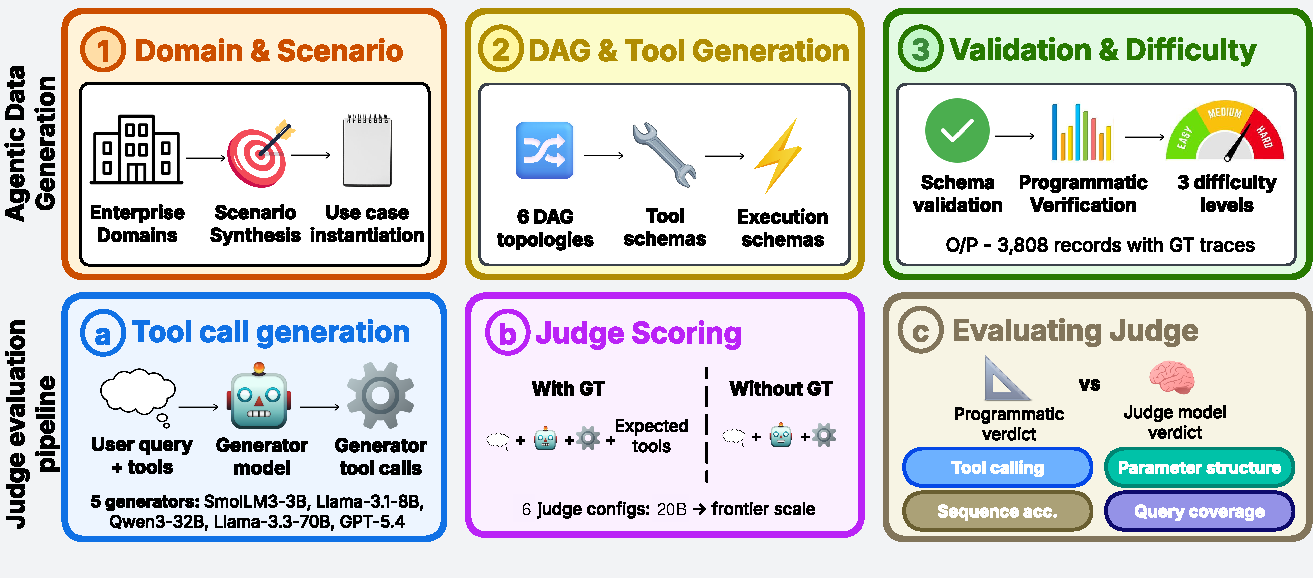
\includegraphics[width=0.75\textwidth]{figures/overall_flow.pdf} \vspace{-0.4cm} \caption{%
    Overall pipeline of AgentJudgeBench. Each BFCL-style Agentic record undergoes difficulty-controlled rewriting, generator inference, and parallel scoring by a programmatic judge and LLM judges (with/without GT), followed by alignment with the programmatic reference.%
  }
  \vspace{-0.3cm}
\label{fig:pipeline}
\end{figure*}

Figure~\ref{fig:pipeline} gives an end-to-end view of the pipeline. Each record is expanded into three difficulty variants; every generator $g \in \mathcal{G}$ produces tool-call predictions; a deterministic programmatic judge scores each prediction to yield a reference vector $\mathbf{p}_r$; and every LLM judge $j \in \mathcal{J}$ produces paired verdicts $\boldsymbol{\ell}^{\text{GT}}_{j,r}$, $\boldsymbol{\ell}^{\text{without GT}}_{j,r}$, compared against $\mathbf{p}_r$ via Eq.~\ref{eq:alignment}.

\vspace{-0.2cm}
\subsection{Data Generation}
\label{sec:methodology:data}
\vspace{-0.1cm}
The benchmark's BFCL-style agentic data is constructed through a multi-stage synthetic pipeline that generates complete agentic records from minimal seed inputs.

\noindent\textbf{Why synthetic.} We generate records synthetically rather than mining real enterprise traces because the two are not interchangeable for this study's purpose. A controlled reliability study needs, for every record, a ground-truth trace we can certify as correct; systematic coverage across dependency structures (six DAG topologies) and difficulty levels (three tiers) rather than whatever distribution happens to occur in logs; and enough scale and domain diversity (15 enterprise domains) to isolate structural effects from domain idiosyncrasy. Real enterprise agentic traces satisfying all three properties are difficult to source: they require access to proprietary internal tool schemas across many domains, live or replayable execution environments, and, for traces to serve as ground truth at all, an independent way to establish that the recorded trace is correct, which is rarely available outside a single organisation's internal systems. Generating records synthetically lets us guarantee a verified reference trace for every one of the $3{,}808$ records and control topology and difficulty independently, which is what makes the paired with-GT/without-GT protocol (\S\ref{sec:methodology:eval}) possible. We do not treat this as cost-free: the Limitations section discusses what a synthetic corpus cannot capture (domain drift, interactive multi-turn execution) and the validation evidence supporting this design choice.

\noindent\textbf{Record construction.} Given an enterprise domain label (e.g., IT service management, contract lifecycle management, energy grid operations), the pipeline generates use-case scenarios, synthesizes a typed tool inventory as function signatures with constrained return types (\texttt{str}, \texttt{bool}, \texttt{list}, \texttt{dict}, \texttt{None}), and produces executable pseudocode linking all tool dependencies. A natural language user utterance is then paired with function input/output specifications, and each function is formalized into a JSON schema with typed arguments, required fields, and output definitions. Finally, an ordered execution trace is produced, capturing sequential and parallel tool calls, their inputs, outputs, and step descriptions.

\noindent\textbf{DAG topologies.} Records are organized into six topologies derived from an analysis of common dependency patterns in real enterprise agentic workflows -- \textit{linear}, \textit{fan-out}, \textit{fan-in}, \textit{diamond}, \textit{optional enrichment}, and \textit{loop-like} -- representing progressively complex dependency structures, from single-path execution to iterative loops.

\noindent\textbf{Difficulty tiers.} Each record is expanded into three levels (\textit{easy}, \textit{medium}, \textit{hard}) by increasing query ambiguity while holding the task structure and GT trace constant. Rewrite validation (Appendix~\ref{app:rewrite-validation}) confirms the medium$\to$hard step on $93.9\%$ of records; the easy$\to$medium step is unanimously validated on only $58.1\%$, and in roughly $41.9\%$ of cases medium is better characterised as a paraphrase than a strict difficulty increase. The primary difficulty-degradation evidence therefore comes from the medium$\to$hard step; medium data should be read as a robustness check rather than a calibrated mid-point (see Limitations~\ref{app:limitations}).

\noindent\textbf{Validation.} GT traces pass a two-level quality gate. First, each record is structurally verified via JSON-schema validation, argument type checking, and trace consistency checks. Second, each (utterance, tool-call) pair is programmatically checked for argument sufficiency, grounding alignment, and query naturalness; failing records are regenerated. No model from $\mathcal{J}$, or any other LLM, is involved in either gate check, ruling out self-reinforcing bias. A 120-record human annotation study on hard-difficulty records (Appendix~\ref{app:prog-judge-validation}), stratified across all six topologies, validates the scorer at $92.7\%$ metric-level agreement with independent human judgement (scope and limitations in Appendix~\ref{app:limitations}). The final corpus comprises $3{,}808$ records spanning 15 enterprise domains with 8--19 tools per record, distributed across six topologies and three difficulty levels.

\vspace{-0.4cm}
\subsection{Evaluation}
\label{sec:methodology:eval}
\vspace{-0.3cm}
As shown in Figure~\ref{fig:eval}, our evaluation is layered: a deterministic \emph{programmatic judge} computes a reference score on every record, an \emph{LLM judge} produces a per-metric verdict on the same record, and an \emph{alignment aggregator} compares the two. Each layer is defined below; symbol definitions appear in Appendix~\ref{app:notation}, and all prompts are reproduced verbatim in Appendix~\ref{app:prompts}.

\noindent\textbf{Programmatic Judge}
\label{sec:methodology:programmatic}

\noindent\textbf{Why a deterministic reference.} The programmatic judge, not a human or LLM annotator, serves as the reference signal against which every LLM judge (and, transitively, the generator) is measured. This is a deliberate choice: the paper's central question is whether LLM judges are reliable, so using another LLM as the reference would reintroduce the same reliability question one level up, and a human-in-the-loop reference cannot scale to the $321{,}648$ evaluations in the full factorial grid. A deterministic, rule-based scorer gives every cell in that grid an identical, reproducible reference. We validate rather than assume this choice: ground-truth traces pass a two-level programmatic quality gate with no LLM involved (below), and a 120-record independent human study (Appendix~\ref{app:prog-judge-validation}) directly checks where the programmatic scorer's notion of correctness agrees and disagrees with human judgement. Let $G = (g_1, \dots, g_{|G|})$ denote the generator's predicted ordered sequence of tool calls and $E = (e_1, \dots, e_{|E|})$ the GT ordered sequence. Let $\mathrm{name}(\cdot)$ return a tool's identifier, $\mathrm{args}(\cdot)$ its argument-key set, and let $\mathcal{G} = \{\mathrm{name}(g_i)\}$, $\mathcal{E} = \{\mathrm{name}(e_i)\}$ denote the unordered sets of tool identifiers. The programmatic judge emits four independent per-record scores in $[0, 1]$. Throughout the paper we call each of these four scores -- tool selection, parameter structure, sequence accuracy, query coverage -- a \emph{metric}: the term denotes one axis of tool-calling correctness scored independently by both the programmatic judge and the LLM judge, not a distinct evaluation instrument or benchmark-level metric.

\textbf{Tool-selection accuracy $p^{\text{tool}}$ and sequence accuracy $p^{\text{seq}}$.}
$p^{\text{tool}}$ penalises set-level mismatch; $p^{\text{seq}}$ measures position-by-position identity, normalised by expected length:

\vspace{-0.4cm}
\begin{subequations}
\small
\begin{align}
p^{\text{tool}}
&=
\max\!\left(
0,\,
1
-
\frac{
|\mathcal{G} \setminus \mathcal{E}|
+
|\mathcal{E} \setminus \mathcal{G}|
}{
\max(|\mathcal{E}|,1)
}
\right)
\label{eq:prog-tool}
\\[6pt]
p^{\text{seq}}
&=
\frac{1}{\max(|E|,1)}
\sum_{i=1}^{\min(|G|,|E|)}
\mathbb{1}\!\left[
\mathrm{name}(g_i)
=
\mathrm{name}(e_i)
\right]
\label{eq:prog-seq}
\end{align}
\vspace{-0.2cm}
\end{subequations}

\noindent with $p^{\text{tool}} = p^{\text{seq}} = 1$ when the respective sequences are empty.

\noindent\textbf{Parameter-structure accuracy $p^{\text{param}}$.}
For each predicted call $g \in G$ let $A_g = \mathrm{args}(g)$ and let $A^{*}_{g}$ be the expected-argument key set of the call in $E$ with the same tool identifier (undefined if the predicted tool is not in $\mathcal{E}$). Define per-call structural scores
\vspace{-0.3cm}
\begin{equation}
\small
\begin{aligned}
s(g)=
\begin{cases}
1.0
& \text{if } A_g = A^{*}_{g}
\\[-1pt]
& \quad \text{(all keys present, no extras)}
\\[4pt]

0.5
& \text{if } A^{*}_{g} \subseteq A_g
\\[-1pt]
& \quad \text{and } A_g \setminus A^{*}_{g} \neq \emptyset
\\[-1pt]
& \quad \text{(extras only)}
\\[4pt]

0.0
& \text{if } A^{*}_{g} \not\subseteq A_g
\\[-1pt]
& \quad \text{or } A^{*}_{g}\ \text{undefined}
\end{cases}
\end{aligned}
\label{eq:prog-param-per-call}
\end{equation}
and aggregate by mean: $p^{\text{param}} = \bigl(\sum_{g \in G} s(g)\bigr) / \max(|G|, 1)$, with $p^{\text{param}} = 1$ when $G$ is empty.

\noindent\textbf{Query-coverage accuracy $p^{\text{cov}}$.}
The fraction of expected tool identifiers covered by the prediction, ignoring extras:
\begin{equation}
p^{\text{cov}} \;=\;
\begin{cases}
  1                                        & \text{if } \mathcal{E} = \emptyset, \\
  0                                        & \text{if } \mathcal{G} \cap \mathcal{E} = \emptyset, \\
  \lvert \mathcal{G} \cap \mathcal{E} \rvert / \lvert \mathcal{E} \rvert & \text{otherwise}.
\end{cases}
\label{eq:prog-cov}
\end{equation}
\noindent\textbf{Record-level aggregate.}
Each record receives a four-element programmatic vector $\mathbf{p}_r = (p^{\text{tool}}_r, p^{\text{param}}_r, p^{\text{seq}}_r, p^{\text{cov}}_r)$. Where a scalar is needed, specifically in the generator-accuracy reporting of Table~\ref{tab:full-results}, we use the unweighted mean $\bar{p}_r = \frac{1}{M} \sum_{m=1}^{M} p^m_r$, where $M=4$ is the number of metrics; elsewhere the four components are kept separate and averaged independently. We adopt equal weights because the four metrics target orthogonal aspects of tool-call correctness and we have no principled basis for preferring one over another when reporting a single headline number; Section~\ref{sec:exp:main} presents per-metric breakdowns that practitioners can reweight for a given application (e.g., upweighting sequence accuracy when judging workflows with strict ordering constraints).
\begin{figure}[t]
  \centering
  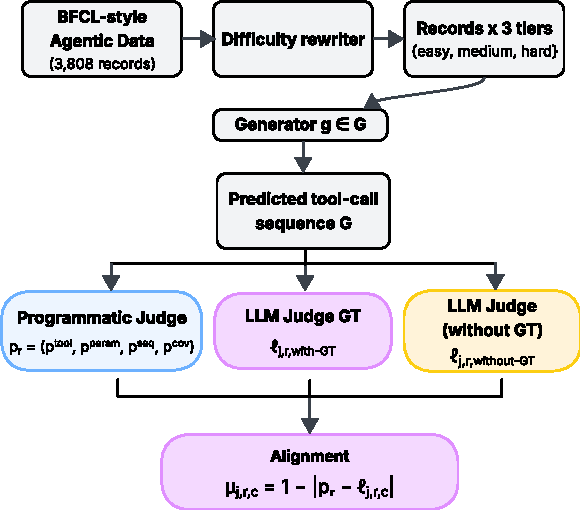
\includegraphics[width=0.95\columnwidth]{figures/Evaluator.pdf} \vspace{-0.1cm}
  \caption{Evaluation pipeline of AgentJudgeBench. Records expand into three difficulty tiers, LLM judges (with/without GT) and programmatic judge score the generated tool-call predictions.}
  \label{fig:eval}
\vspace{-0.4cm}
\end{figure}
Empirically, the judge ranking is stable under alternative metric weightings: Spearman $\rho \geq 0.83$\footnote{Spearman's $\rho$ is a rank correlation coefficient measuring the monotone association between two orderings; $\rho=1$ indicates identical rankings, $\rho=0$ no association, and $\rho=-1$ perfectly reversed rankings.} between the equal-weight ranking and five alternative schemes (seq${\times}2$, param${\times}2$, cov${\times}0.5$, seq${\times}2{+}$param${\times}2$), confirming that the equal-weight aggregate is an adequate proxy for any practitioner-specific weighting.

\noindent\textbf{LLM Judge}
\label{sec:methodology:llmjudge}
The same generator outputs scored by the programmatic judge are independently evaluated by every LLM judge $j \in \mathcal{J}$. Each judge receives a structured prompt containing the original user query, the full set of available tool schemas, and the generator's predicted tool-call sequence, and is asked to produce a single JSON object scoring each of the four metrics (tool selection, parameter structure, sequence accuracy, query coverage) on a $\{0, 0.5, 1\}$ scale, along with a one-sentence justification per metric and an overall assessment.

Two prompt variants exist, corresponding to the conditions $c \in \{\text{with-GT}, \text{without-GT}\}$: the \textbf{with-GT} prompt additionally exposes the GT tool-call sequence as a reference block, while the \textbf{without-GT} prompt omits it entirely, requiring the judge to assess correctness from the query and tool schemas alone. Judge decoding is held constant across all $(g, j, d, c)$ configurations to isolate the effect of our independent variables. The full prompt bodies appear in Appendix~\ref{app:prompts}.

\noindent\textbf{Alignment Against the Programmatic Reference}
\label{sec:methodology:alignment}
Given a record $r$, condition $c$, judge $j$, and metric $m \in \{\text{tool}, \text{param}, \text{seq}, \text{cov}\}$, let $\ell^{m}_{j,r,c} \in \{0, 0.5, 1\}$ denote the judge's verdict and $p^{m}_r$ the programmatic value. The per-metric match score and record-level aggregate are:
\vspace{-0.2cm}
\begin{subequations}
\begin{align}
\mu^{m}_{j,r,c}
&=
1 - \left| p^{m}_r - \ell^{m}_{j,r,c} \right|
\label{eq:per-metric-match}
\\[4pt]
\mu_{j,r,c}
&=
\frac{1}{M}
\sum_{m=1}^{M}
\mu^{m}_{j,r,c}
\label{eq:overall_alignment}
\end{align}
\end{subequations}
\noindent exact match on all metrics yields $\mu = 1$ and maximally divergent verdict yields $0$. The configuration-level alignment percentage and GT lift are:
\vspace{-0.2cm}
\begin{subequations}
\begin{align}
\mathrm{align}(j, g, d, c)
&=
\frac{100}{N_{g,d}}
\sum_{r=1}^{N_{g,d}}
\mu_{j,r,c}
\label{eq:alignment}
\\[4pt]
\mathrm{lift}(j)
&=
\overline{\mathrm{align}}_{\text{GT}}(j)
-
\overline{\mathrm{align}}_{\text{without GT}}(j)
\label{eq:lift}
\end{align}
\end{subequations}
\noindent where the overline denotes the mean over all 12 $(g, d)$ configurations. Perfect reproduction of the programmatic vector yields $\mathrm{align} = 100\%$; an independent judge attains $50\%$ in expectation.

In the experiments, we report both aggregate alignment $\mathrm{align}(j, g, d, c)$ and per-metric breakdowns to identify which dimensions of tool-calling correctness judges find most difficult to assess.